\documentclass{standalone}
\usepackage{tikz}
\usetikzlibrary{shapes.geometric, arrows.meta, positioning, calc, fit, backgrounds, decorations.pathreplacing}
\hyphenpenalty=10000
\exhyphenpenalty=10000

% ==============================================================================
% COLOR PALETTE (Strict Academic Color Harmony - Verified RISC/FPGA Architecture Style)
% ==============================================================================
% 1. Module Fill Colors (Unified Rich Gold "Batata" with crisp pure black outline)
\definecolor{boxFill}{HTML}{F5BC01}              % Rich Gold (#F5BC01) matching Poster Identity
\definecolor{boxBorder}{RGB}{0, 0, 0}            % Pure crisp pitch black (#000000) for bold outlines
\definecolor{boxTitle}{RGB}{0, 0, 0}            % Pure crisp black for module title
\definecolor{navyDark}{HTML}{0F2B5C}             % Prestigious Dark Navy Blue (#0F2B5C) matching Poster Identity
\definecolor{navyMid}{HTML}{1E3A8A}              % Navy accent
\definecolor{borderGray}{HTML}{CBD5E1}           % Border gray

% 2. Stage Enclosure Backgrounds & Boundary Frames
\definecolor{stageBlueBg}{RGB}{240, 246, 255}
\definecolor{stageBlueFrame}{RGB}{2, 132, 199}  % Sky blue stage frame
\definecolor{stageAmberBg}{RGB}{255, 251, 235}
\definecolor{stageAmberFrame}{RGB}{217, 119, 6} % Amber stage frame (>55% Area Core)
\definecolor{stagePurpleBg}{RGB}{245, 243, 255}
\definecolor{stagePurpleFrame}{RGB}{124, 58, 237}% Purple stage frame
\definecolor{boundaryBlack}{RGB}{15, 23, 42}   % Top-Level Entity Boundary (Solid Authoritative Black)

% 3. Semantic Wire & Signal Routing Colors
\definecolor{wireBlue}{RGB}{2, 105, 215}      % Address / Tag / Sub-block (32b / 24b / 6b / 137b)
\definecolor{wireRed}{RGB}{220, 20, 30}       % 256b Data Bus / Match / Evict / Refill
\definecolor{wireOrange}{RGB}{235, 110, 0}    % Write Enables / Clock / Tag Compare / PLRU
\definecolor{wireGreen}{RGB}{10, 140, 50}     % Valid Flags / Hit / Way-Enable / STLF Valid
\definecolor{wireMagenta}{RGB}{205, 10, 120}  % Selection / BDI Code / Compressed Payload
\definecolor{wireSlate}{RGB}{55, 65, 80}      % Internal Intermediate Vectors

% 4. Connection Pin Dots (100% Matching Semantic Wire Colors)
\definecolor{pinBlue}{RGB}{2, 105, 215}
\definecolor{pinRed}{RGB}{220, 20, 30}
\definecolor{pinOrange}{RGB}{235, 110, 0}
\definecolor{pinGreen}{RGB}{10, 140, 50}
\definecolor{pinMagenta}{RGB}{205, 10, 120}
\definecolor{pinSlate}{RGB}{55, 65, 80}

\tikzset{
  % Standardized Hardware Module Style: Pure Black 1.8pt Outline with Rich Gold Fill
  hwmodule/.style={
    draw=boxBorder,
    line width=1.8pt,
    fill=boxFill,
    rounded corners=3.5pt,
    minimum width=3.8cm,
    minimum height=1.85cm,
    text width=3.7cm,
    align=center,
    font=\small\bfseries,
    text=boxTitle,
    inner sep=3pt
  },
  % Hero Block Style - Thick 2.2pt Black Border
  heromodule/.style={
    draw=boxBorder,
    line width=2.2pt,
    fill=boxFill,
    rounded corners=4.5pt,
    align=center,
    font=\small\bfseries,
    text=boxTitle,
    inner sep=4pt
  },
  % Stage Group Background Boundary Style
  stagegroup/.style={
    draw=#1,
    line width=1.6pt,
    rounded corners=7pt,
    fill=#1!4!white,
    inner sep=10pt
  },
  % Connection Pin Dots
  pDot/.style={
    circle,
    fill=#1,
    draw=black!95!white,
    line width=0.8pt,
    inner sep=2.2pt
  },
  % Wire Junction Dots
  jDot/.style={
    circle,
    fill=#1,
    inner sep=2.4pt
  },
  % Manhattan Orthogonal Wire Styles with prominent arrowheads
  wBlue/.style={line width=1.8pt, draw=wireBlue, ->, >={Latex[length=2.8mm, width=2.0mm]}},
  wRed/.style={line width=1.8pt, draw=wireRed, ->, >={Latex[length=2.8mm, width=2.0mm]}},
  wOrange/.style={line width=1.7pt, draw=wireOrange, ->, >={Latex[length=2.8mm, width=2.0mm]}},
  wGreen/.style={line width=1.7pt, draw=wireGreen, ->, >={Latex[length=2.8mm, width=2.0mm]}},
  wMagenta/.style={line width=1.7pt, draw=wireMagenta, ->, >={Latex[length=2.8mm, width=2.0mm]}},
  wSlate/.style={line width=1.7pt, draw=wireSlate, ->, >={Latex[length=2.8mm, width=2.0mm]}},
  % Solid Rich Badges
  badge/.style={
    font=\sffamily\bfseries\footnotesize,
    rounded corners=2.5pt,
    inner sep=2.2pt,
    draw=black!90!white,
    line width=0.7pt,
    text=white
  },
  badgeC/.style={badge, fill=wireBlue!95!black},
  badgeR/.style={badge, fill=wireRed!95!black},
  badgeO/.style={badge, fill=wireOrange!95!black},
  badgeG/.style={badge, fill=wireGreen!90!black},
  badgeM/.style={badge, fill=wireMagenta!90!black},
  badgeK/.style={badge, fill=wireSlate!95!black}
}

\begin{document}
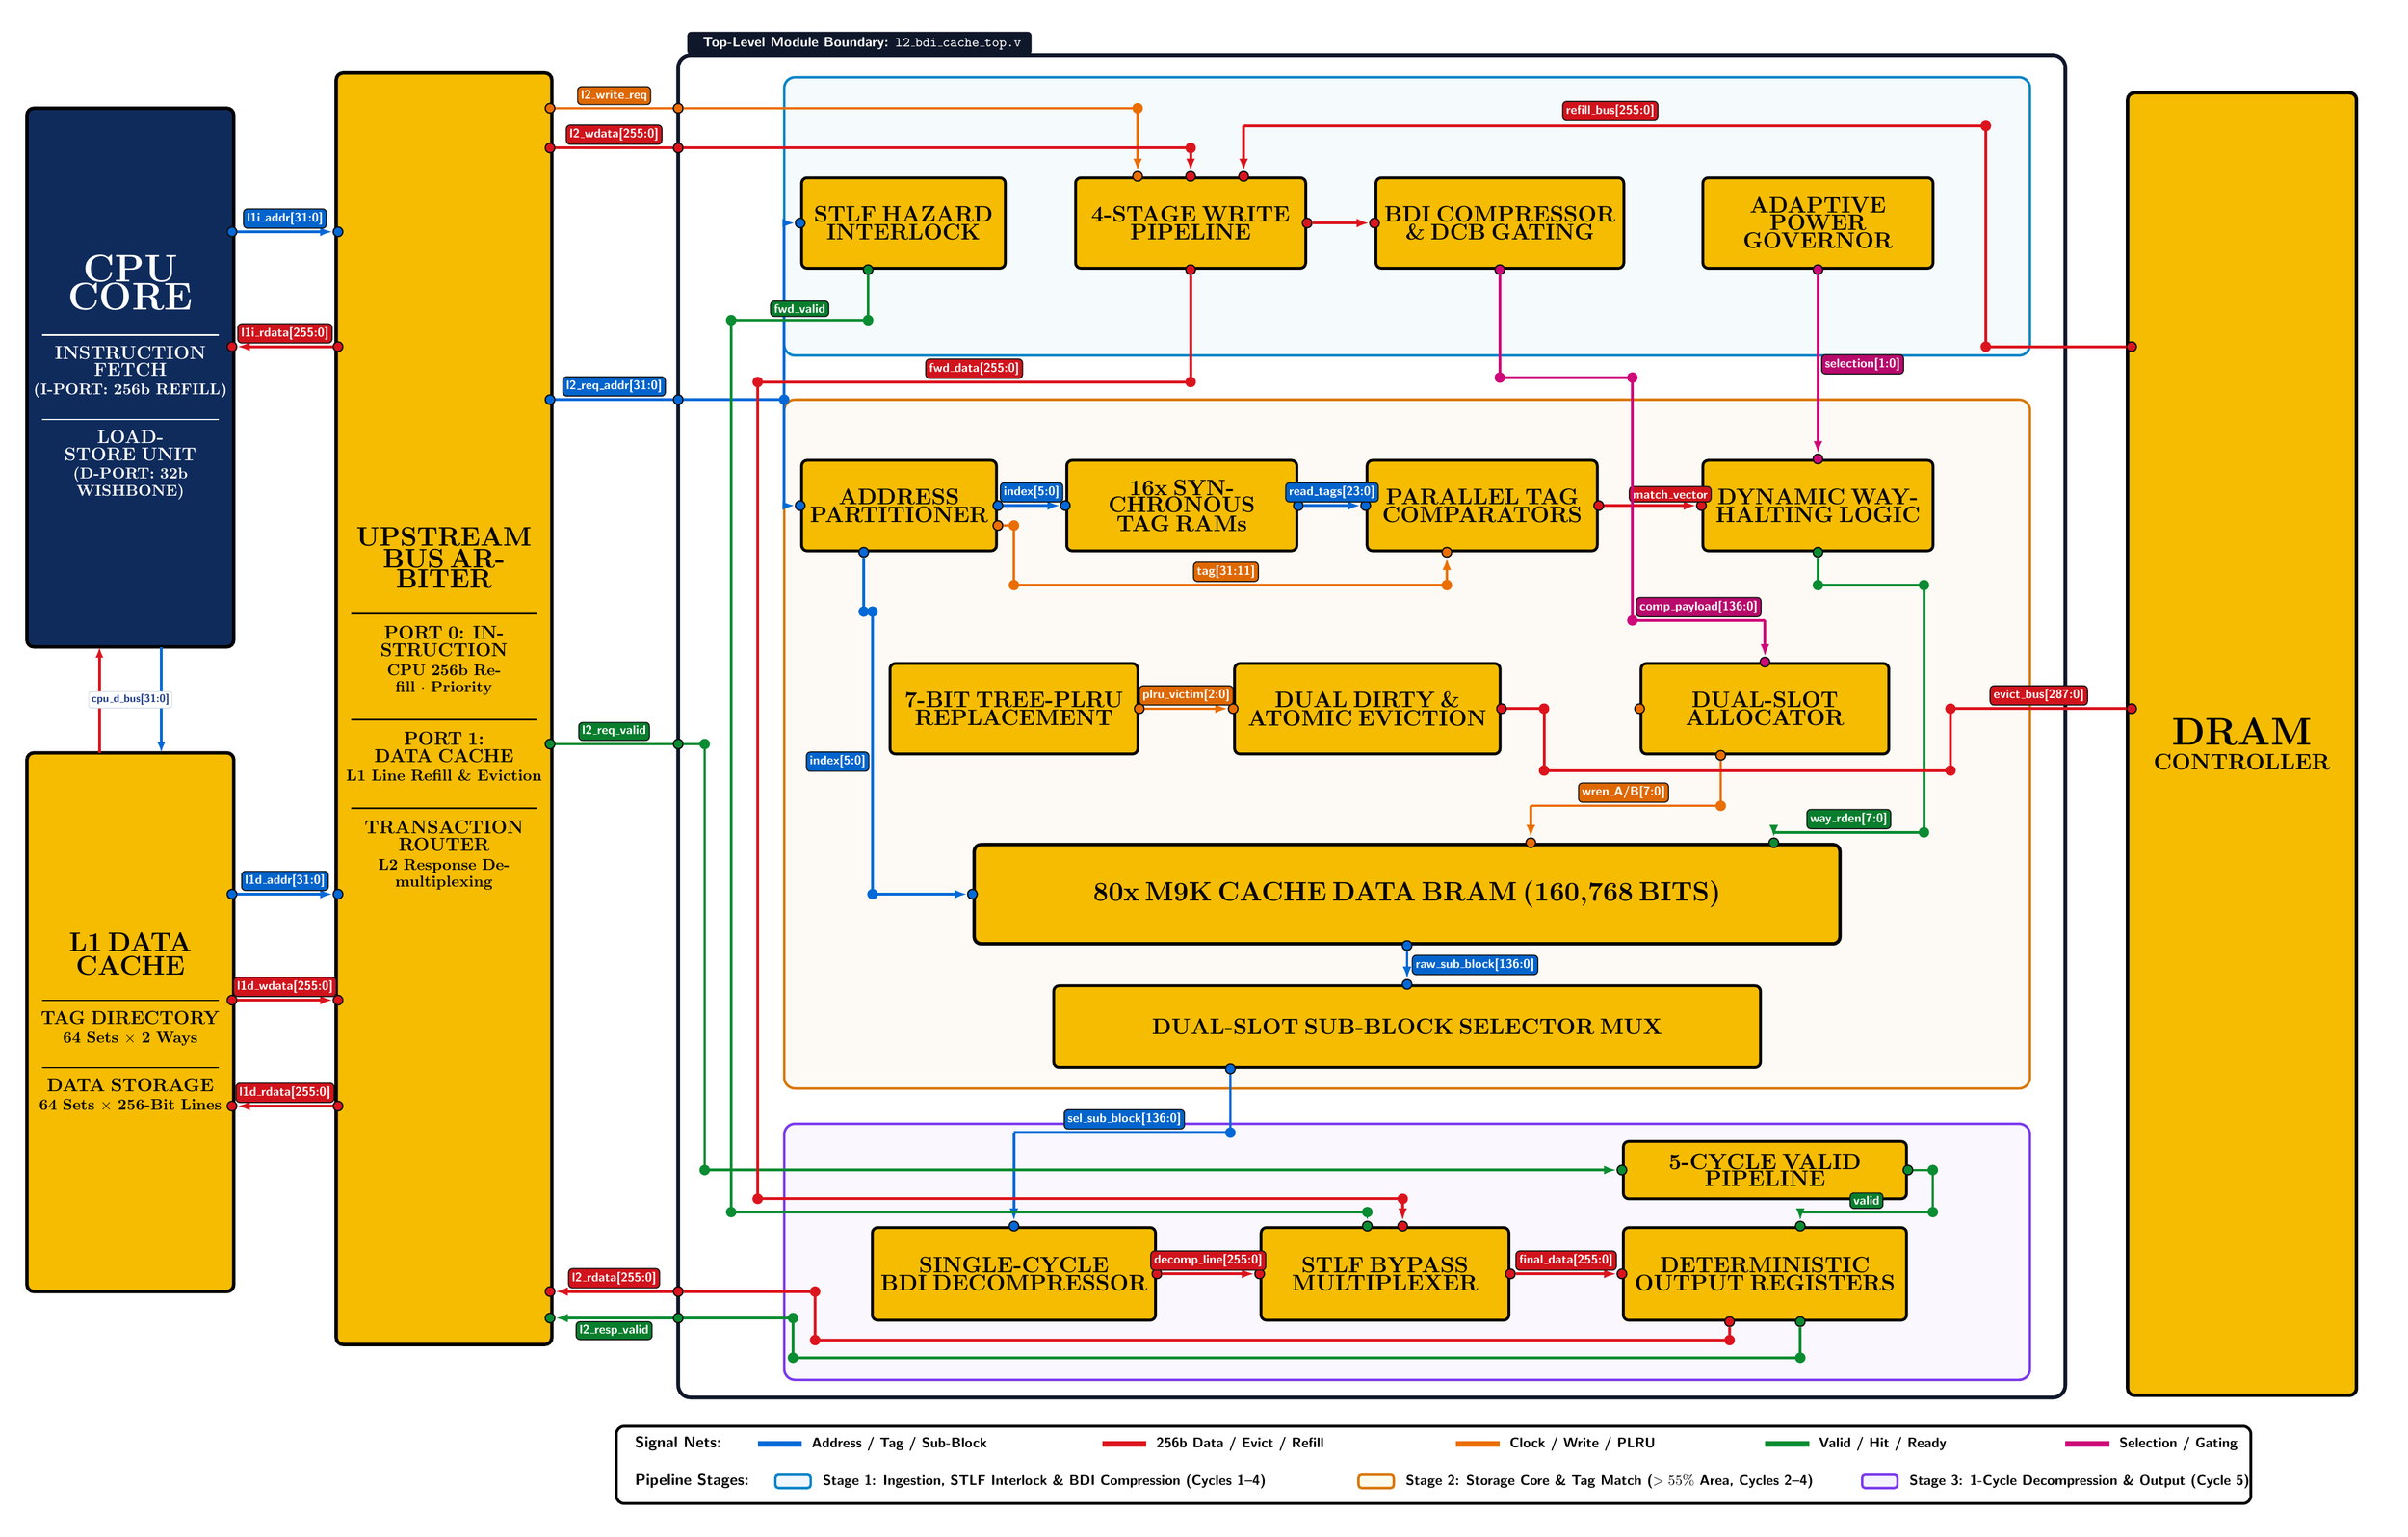
\begin{tikzpicture}[
  x=1cm, y=1cm,
  >=Stealth,
  node distance=0.8cm,
  font=\sffamily
]

% ==============================================================================
% CANVAS BOUNDING BOX & BACKGROUND
% Generous width from X = -14.6 to 39.2 accommodating Host Hierarchy & Arbiter
% ==============================================================================
\path[use as bounding box] (-14.60, -5.60) rectangle (39.20, 28.50);
\fill[white] (-14.60, -5.60) rectangle (39.20, 28.50);

% ==============================================================================
% MASTER MAGENTA ENCLOSURE (Top-Level Entity Boundary: l2_bdi_cache_top.v)
% Encloses L2 Subsystem ONLY (from X = 1.0 to 31.8).
% All external transactions enter horizontally with zero vertical wire crowding!
% ==============================================================================
\draw[boundaryBlack, line width=2.4pt, rounded corners=8pt]
  (0.4, -2.8) rectangle (31.8, 27.6);
\node[fill=boundaryBlack, text=white, font=\sffamily\bfseries\small, rounded corners=2.5pt, anchor=south west] 
  at (0.6, 27.6) {\ \ Top-Level Module Boundary: \texttt{l2\_bdi\_cache\_top.v}\ \ };

% ==============================================================================
% 1. HOST TIER COLUMN 1: RISC-V CPU CORE & LEVEL-1 DATA CACHE
% ==============================================================================
% (A) CPU Core (Top Left - Navy Blue Fill with Crisp White Text)
\node[heromodule, fill=navyDark, text=white, minimum width=4.6cm, minimum height=12.2cm, text width=4.4cm] (cpu_core) at (-12.0, 20.3) {
  \textbf{\Huge CPU CORE}\\[1.4ex]
  \rule{4.0cm}{0.9pt}\\[1.0ex]
  \textbf{\large INSTRUCTION FETCH}\\[0.2ex]
  \textbf{\normalsize (I-PORT: 256b REFILL)}\\[1.4ex]
  \rule{4.0cm}{0.9pt}\\[1.0ex]
  \textbf{\large LOAD-STORE UNIT}\\[0.2ex]
  \textbf{\normalsize (D-PORT: 32b WISHBONE)}
};

% (B) Level-1 Data Cache (Bottom Left - Rich Gold Fill)
\node[heromodule, fill=boxFill, minimum width=4.6cm, minimum height=12.2cm, text width=4.4cm] (l1_cache) at (-12.0, 5.7) {
  \textbf{\LARGE L1 DATA}\\[0.5ex]
  \textbf{\LARGE CACHE}\\[1.5ex]
  \rule{4.0cm}{0.9pt}\\[1.0ex]
  \textbf{\large TAG DIRECTORY}\\[0.2ex]
  \textbf{\normalsize 64 Sets $\times$ 2 Ways}\\[1.4ex]
  \rule{4.0cm}{0.9pt}\\[1.0ex]
  \textbf{\large DATA STORAGE}\\[0.2ex]
  \textbf{\normalsize 64 Sets $\times$ 256-Bit Lines}
};

% Processor LSU to L1 Data Cache Interconnect (Pure Straight Vertical Bus)
\draw[line width=1.8pt, draw=wireBlue, ->, >={Latex[length=2.4mm, width=1.8mm]}] (-11.3, 14.2) -- (-11.3, 11.8);
\draw[line width=1.8pt, draw=wireRed, ->, >={Latex[length=2.4mm, width=1.8mm]}] (-12.7, 11.8) -- (-12.7, 14.2);
\node[font=\sffamily\bfseries\scriptsize, text=navyMid, fill=white, inner sep=1.8pt, rounded corners=1.5pt, draw=borderGray] at (-12.0, 13.0) {cpu\_d\_bus[31:0]};

% ==============================================================================
% 2. HOST TIER COLUMN 2: UPSTREAM BUS ARBITER (Matching Research Paper Fig 1)
% Strictly arbitrates between CPU Instruction Fetch & L1 Data Cache Line Accesses
% ==============================================================================
\node[heromodule, fill=boxFill, minimum width=4.8cm, minimum height=28.8cm, text width=4.6cm] (arbiter) at (-4.9, 12.8) {
  \textbf{\LARGE UPSTREAM}\\[0.3ex]
  \textbf{\LARGE BUS ARBITER}\\[1.6ex]
  \rule{4.2cm}{1.2pt}\\[1.2ex]
  \textbf{\large PORT 0: INSTRUCTION}\\[0.3ex]
  \textbf{\normalsize CPU 256b Refill $\cdot$ Priority}\\[1.8ex]
  \rule{4.2cm}{1.2pt}\\[1.2ex]
  \textbf{\large PORT 1: DATA CACHE}\\[0.3ex]
  \textbf{\normalsize L1 Line Refill \& Eviction}\\[1.8ex]
  \rule{4.2cm}{1.2pt}\\[1.2ex]
  \textbf{\large TRANSACTION ROUTER}\\[0.3ex]
  \textbf{\normalsize L2 Response Demultiplexing}
};

% Interconnects from CPU / L1 to Arbiter (Wide 2.4cm channel: X = -9.7 to -7.3)
% CPU I-Fetch -> Arbiter Port 0
\node[pDot=pinBlue] (p_cpu_ifetch_a) at (-9.7, 23.6) {};
\node[pDot=pinBlue] (p_arb_p0_in) at (-7.3, 23.6) {};
\draw[wBlue] (p_cpu_ifetch_a) -- node[above=2pt, badgeC]{l1i\_addr[31:0]} (p_arb_p0_in);

\node[pDot=pinRed] (p_arb_p0_out) at (-7.3, 21.0) {};
\node[pDot=pinRed] (p_cpu_ifetch_d) at (-9.7, 21.0) {};
\draw[wRed] (p_arb_p0_out) -- node[above=2pt, badgeR]{l1i\_rdata[255:0]} (p_cpu_ifetch_d);

% L1 Data Cache -> Arbiter Port 1
\node[pDot=pinBlue] (p_l1_req_a) at (-9.7, 8.6) {};
\node[pDot=pinBlue] (p_arb_p1_in_a) at (-7.3, 8.6) {};
\draw[wBlue] (p_l1_req_a) -- node[above=2pt, badgeC]{l1d\_addr[31:0]} (p_arb_p1_in_a);

\node[pDot=pinRed] (p_l1_req_d) at (-9.7, 6.2) {};
\node[pDot=pinRed] (p_arb_p1_in_d) at (-7.3, 6.2) {};
\draw[wRed] (p_l1_req_d) -- node[above=2pt, badgeR]{l1d\_wdata[255:0]} (p_arb_p1_in_d);

\node[pDot=pinRed] (p_arb_p1_out_d) at (-7.3, 3.8) {};
\node[pDot=pinRed] (p_l1_resp_d) at (-9.7, 3.8) {};
\draw[wRed] (p_arb_p1_out_d) -- node[above=2pt, badgeR]{l1d\_rdata[255:0]} (p_l1_resp_d);

% ==============================================================================
% 3. RIGHT COLUMN: OFF-CHIP DRAM CONTROLLER
% Height matched to 29.5cm exactly matching the Left Host Column!
% ==============================================================================
\node[heromodule, minimum width=5.0cm, minimum height=29.5cm, text width=4.9cm] (dram) at (35.8, 12.0) {
  \textbf{\Huge DRAM}\\[1.2ex]
  \textbf{\Large CONTROLLER}
};

% ==============================================================================
% STAGE 1: FRONTEND, STLF HAZARD INTERLOCK & COMPRESSION PIPELINE (Y: 20.8 to 27.1)
% ==============================================================================
\draw[stagegroup=stageBlueFrame] (2.8, 20.8) rectangle (31.0, 27.1);

% Stage 1 Modules: Pure Single Titles with Crisp 1.8pt Black Outlines
\node[hwmodule, minimum width=4.6cm, minimum height=2.05cm, text width=4.4cm] (stlf) at (5.5, 23.8) {
  \textbf{\Large STLF HAZARD}\\[0.2ex]
  \textbf{\Large INTERLOCK}
};

\node[hwmodule, minimum width=5.2cm, minimum height=2.05cm, text width=5.0cm] (wpipe) at (12.0, 23.8) {
  \textbf{\Large 4-STAGE WRITE}\\[0.2ex]
  \textbf{\Large PIPELINE}
};

\node[hwmodule, minimum width=5.6cm, minimum height=2.05cm, text width=5.4cm] (bdi_comp) at (19.0, 23.8) {
  \textbf{\Large BDI COMPRESSOR}\\[0.2ex]
  \textbf{\Large \& DCB GATING}
};

\node[hwmodule, minimum width=5.2cm, minimum height=2.05cm, text width=5.0cm] (governor) at (26.2, 23.8) {
  \textbf{\Large ADAPTIVE POWER}\\[0.2ex]
  \textbf{\Large GOVERNOR}
};

% Stage 1 Pin Dots
\node[pDot=pinBlue] (pin_stlf_w) at (stlf.west) {};
\node[pDot=pinGreen] (pin_stlf_s) at ($(stlf.south)+(-0.8,0)$) {};

\node[pDot=pinOrange] (pin_wpipe_n_wr) at ($(wpipe.north)+(-1.2,0)$) {};
\node[pDot=pinRed] (pin_wpipe_n_data) at (wpipe.north) {};
\node[pDot=pinRed] (pin_wpipe_n_refill) at ($(wpipe.north)+(1.2,0)$) {};
\node[pDot=pinRed] (pin_wpipe_e) at (wpipe.east) {};
\node[pDot=pinRed] (pin_wpipe_s) at (wpipe.south) {};

\node[pDot=pinRed] (pin_bdi_w) at (bdi_comp.west) {};
\node[pDot=pinMagenta] (pin_bdi_s) at (bdi_comp.south) {};

\node[pDot=pinMagenta] (pin_gov_s) at (governor.south) {};

% ==============================================================================
% STAGE 2: CACHE STORAGE CORE (>55% CANVAS AREA, Y: 4.2 to 19.8)
% ==============================================================================
\draw[stagegroup=stageAmberFrame] (2.8, 4.2) rectangle (31.0, 19.8);

% ROW 1 (Y = 17.4): Tag Pipeline & Power Gating
\node[hwmodule, minimum width=4.4cm, minimum height=2.05cm, text width=4.2cm] (addr_split) at (5.4, 17.4) {
  \textbf{\Large ADDRESS}\\[0.2ex]
  \textbf{\Large PARTITIONER}
};

\node[hwmodule, minimum width=5.2cm, minimum height=2.05cm, text width=5.0cm] (tag_ram) at (11.8, 17.4) {
  \textbf{\Large 16x SYNCHRONOUS}\\[0.3ex]
  \textbf{\Large TAG RAMs}
};

\node[hwmodule, minimum width=5.2cm, minimum height=2.05cm, text width=5.0cm] (tag_cmp) at (18.6, 17.4) {
  \textbf{\Large PARALLEL TAG}\\[0.2ex]
  \textbf{\Large COMPARATORS}
};

\node[hwmodule, minimum width=5.2cm, minimum height=2.05cm, text width=5.0cm] (way_halt) at (26.2, 17.4) {
  \textbf{\Large DYNAMIC WAY-}\\[0.2ex]
  \textbf{\Large HALTING LOGIC}
};

% Pins for Row 1
\node[pDot=pinBlue] (pin_addr_split_w) at (addr_split.west) {};
\node[pDot=pinBlue] (pin_addr_split_e_idx) at (addr_split.east) {};
\node[pDot=pinOrange] (pin_addr_split_e_tag) at ($(addr_split.east)+(0,-0.45)$) {};
\node[pDot=pinBlue] (pin_addr_split_s) at ($(addr_split.south)+(-0.8,0)$) {};

\node[pDot=pinBlue] (pin_tag_ram_w) at (tag_ram.west) {};
\node[pDot=pinBlue] (pin_tag_ram_e) at (tag_ram.east) {};

\node[pDot=pinBlue] (pin_tag_cmp_w) at (tag_cmp.west) {};
\node[pDot=pinOrange] (pin_tag_cmp_s) at ($(tag_cmp.south)+(-0.8,0)$) {};
\node[pDot=pinRed] (pin_tag_cmp_e) at (tag_cmp.east) {};

\node[pDot=pinRed] (pin_way_halt_w) at (way_halt.west) {};
\node[pDot=pinMagenta] (pin_way_halt_n) at (way_halt.north) {};
\node[pDot=pinGreen] (pin_way_halt_s) at (way_halt.south) {};

% Row 1 Direct Interconnects
\draw[wBlue] (pin_addr_split_e_idx) -- node[above=2pt, badgeC]{index[5:0]} (pin_tag_ram_w);
\draw[wBlue] (pin_tag_ram_e) -- node[above=2pt, badgeC]{read\_tags[23:0]} (pin_tag_cmp_w);
\draw[wRed] (pin_tag_cmp_e) -- node[pos=0.72, above=2pt, badgeR]{match\_vector} (pin_way_halt_w);

% Tag compare bypass wire: addr_split -> tag_cmp.south
\draw[line width=1.6pt, draw=wireOrange] (pin_addr_split_e_tag) -- (8.0, 16.95) -- (8.0, 15.6) -- (17.8, 15.6);
\node[jDot=wireOrange] at (8.0, 16.95) {};
\node[jDot=wireOrange] at (8.0, 15.6) {};
\node[jDot=wireOrange] at (17.8, 15.6) {};
\node[badgeO, above=2pt] at (12.8, 15.6) {tag[31:11]};
\draw[wOrange] (17.8, 15.6) -- (pin_tag_cmp_s);

% ROW 2 (Y = 12.8): Replacement, Dirty Eviction & Dual-Slot Formatting
\node[hwmodule, minimum width=5.6cm, minimum height=2.05cm, text width=5.4cm] (plru) at (8.0, 12.8) {
  \textbf{\Large 7-BIT TREE-PLRU}\\[0.2ex]
  \textbf{\Large REPLACEMENT}
};

\node[hwmodule, minimum width=6.0cm, minimum height=2.05cm, text width=5.8cm] (dirty_evict) at (16.0, 12.8) {
  \textbf{\Large DUAL DIRTY \&}\\[0.2ex]
  \textbf{\Large ATOMIC EVICTION}
};

\node[hwmodule, minimum width=5.6cm, minimum height=2.05cm, text width=5.4cm] (sub_alloc) at (25.0, 12.8) {
  \textbf{\Large DUAL-SLOT}\\[0.2ex]
  \textbf{\Large ALLOCATOR}
};

% Pins for Row 2
\node[pDot=pinOrange] (pin_plru_e) at (plru.east) {};
\node[pDot=pinOrange] (pin_dirty_w) at (dirty_evict.west) {};
\node[pDot=pinRed] (pin_dirty_e) at (dirty_evict.east) {};

\node[pDot=pinOrange] (pin_sub_alloc_w) at (sub_alloc.west) {};
\node[pDot=pinMagenta] (pin_sub_alloc_n) at (sub_alloc.north) {};
\node[pDot=pinOrange] (pin_sub_alloc_s) at ($(sub_alloc.south)+(-1.0,0)$) {};

% Row 2 Interconnects
\draw[wOrange] (pin_plru_e) -- node[above=2pt, badgeO]{plru\_victim[2:0]} (pin_dirty_w);

% ROW 3 (Y = 8.6): HERO BLOCK - 80x M9K Cache Storage BRAM (160,768 Bits)
\node[heromodule, minimum width=19.6cm, minimum height=2.25cm, text width=19.2cm] (data_bram) at (16.9, 8.6) {
  \textbf{\LARGE 80x M9K CACHE DATA BRAM (160,768 BITS)}
};

% Pins for Data BRAM
\node[pDot=pinBlue] (pin_data_bram_w) at (data_bram.west) {};
\node[pDot=pinGreen] (pin_data_bram_n_rd) at ($(data_bram.north)+(8.3,0)$) {};
\node[pDot=pinOrange] (pin_data_bram_n_wr) at ($(data_bram.north)+(2.8,0)$) {};
\node[pDot=pinBlue] (pin_data_bram_s) at (data_bram.south) {};

% ROW 4 (Y = 5.6): Dual-Slot Sub-Block Selector MUX
\node[hwmodule, minimum width=16.0cm, minimum height=1.85cm, text width=15.6cm] (sub_mux) at (16.9, 5.6) {
  \textbf{\Large DUAL-SLOT SUB-BLOCK SELECTOR MUX}
};

% Pins for Sub-Block Selector Mux
\node[pDot=pinBlue] (pin_sub_mux_n) at (sub_mux.north) {};
\node[pDot=pinBlue] (pin_sub_mux_s) at ($(sub_mux.south)+(-4.0,0)$) {};

% Inter-Row Connections in Stage 2
% Level 1: Way Halting -> Data BRAM read enables (Routed through clear eastern corridor at X = 28.6, ZERO box penetration!)
\draw[line width=1.7pt, draw=wireGreen] (pin_way_halt_s) -- (26.2, 15.6) -- (28.6, 15.6) -- (28.6, 10.0) -- (25.2, 10.0);
\node[jDot=wireGreen] at (26.2, 15.6) {};
\node[jDot=wireGreen] at (28.6, 15.6) {};
\node[jDot=wireGreen] at (28.6, 10.0) {};
\node[badgeG, above=2pt] at (26.9, 10.0) {way\_rden[7:0]};
\draw[wGreen] (25.2, 10.0) -- (pin_data_bram_n_rd);

% Level 2: Dual-Slot Allocator -> Data BRAM write enables at Y = 10.6 (Clean, above BRAM top, zero border collision!)
\draw[line width=1.7pt, draw=wireOrange] (pin_sub_alloc_s) -- (24.0, 10.6) -- (19.7, 10.6);
\node[jDot=wireOrange] at (24.0, 10.6) {};
\node[badgeO, above=2pt] at (21.8, 10.6) {wren\_A/B[7:0]};
\draw[wOrange] (19.7, 10.6) -- (pin_data_bram_n_wr);

% Data BRAM -> Sub-Block MUX
\draw[wBlue] (pin_data_bram_s) -- node[right=3pt, badgeC]{raw\_sub\_block[136:0]} (pin_sub_mux_n);

% ==============================================================================
% STAGE 3: DECOMPRESSION & DETERMINISTIC 5-CYCLE OUTPUT PIPELINE (Y: -2.4 to 3.4)
% ==============================================================================
\draw[stagegroup=stagePurpleFrame] (2.8, -2.4) rectangle (31.0, 3.4);

% Control: 5-Cycle Valid Shift Register
\node[hwmodule, minimum width=6.4cm, minimum height=1.30cm, text width=6.2cm] (valid_pipe) at (25.0, 2.35) {
  \textbf{\Large 5-CYCLE VALID PIPELINE}
};

% Datapath Modules at Y = 0.0
\node[hwmodule, minimum width=6.4cm, minimum height=2.10cm, text width=6.2cm] (decompress) at (8.0, 0.0) {
  \textbf{\Large SINGLE-CYCLE}\\[0.2ex]
  \textbf{\Large BDI DECOMPRESSOR}
};

\node[hwmodule, minimum width=5.6cm, minimum height=2.10cm, text width=5.4cm] (stlf_mux) at (16.4, 0.0) {
  \textbf{\Large STLF BYPASS}\\[0.2ex]
  \textbf{\Large MULTIPLEXER}
};

\node[hwmodule, minimum width=6.4cm, minimum height=2.10cm, text width=6.2cm] (out_regs) at (25.0, 0.0) {
  \textbf{\Large DETERMINISTIC}\\[0.2ex]
  \textbf{\Large OUTPUT REGISTERS}
};

% Stage 3 Pins
\node[pDot=pinGreen] (pin_valid_pipe_w) at (valid_pipe.west) {};
\node[pDot=pinGreen] (pin_valid_pipe_e) at (valid_pipe.east) {};

\node[pDot=pinBlue] (pin_decomp_n) at (decompress.north) {};
\node[pDot=pinRed] (pin_decomp_e) at (decompress.east) {};

\node[pDot=pinRed] (pin_stlf_mux_w) at (stlf_mux.west) {};
\node[pDot=pinRed] (pin_stlf_mux_n_dat) at ($(stlf_mux.north)+(0.4,0)$) {};
\node[pDot=pinGreen] (pin_stlf_mux_n_val) at ($(stlf_mux.north)+(-0.4,0)$) {};
\node[pDot=pinRed] (pin_stlf_mux_e) at (stlf_mux.east) {};

\node[pDot=pinRed] (pin_out_regs_w) at (out_regs.west) {};
\node[pDot=pinGreen] (pin_out_regs_n) at ($(out_regs.north)+(0.8,0)$) {};
\node[pDot=pinRed] (pin_out_regs_s_data) at ($(out_regs.south)+(-0.8,0)$) {};
\node[pDot=pinGreen] (pin_out_regs_s) at ($(out_regs.south)+(0.8,0)$) {};

% Stage 3 Horizontal Connections
\draw[wRed] (pin_decomp_e) -- node[above=2pt, badgeR]{decomp\_line[255:0]} (pin_stlf_mux_w);
\draw[wRed] (pin_stlf_mux_e) -- node[above=2pt, badgeR]{final\_data[255:0]} (pin_out_regs_w);

% Valid Pipe to Output Registers
\draw[line width=1.6pt, draw=wireGreen] (pin_valid_pipe_e) -- (28.8, 2.35) -- (28.8, 1.4) -- (25.8, 1.4);
\node[jDot=wireGreen] at (28.8, 2.35) {};
\node[jDot=wireGreen] at (28.8, 1.4) {};
\node[badgeG, above=2pt] at (27.3, 1.4) {valid};
\draw[wGreen] (25.8, 1.4) -- (pin_out_regs_n);

% Sub-block Mux to Decompressor
\draw[line width=1.7pt, draw=wireBlue] (pin_sub_mux_s) -- (12.9, 3.2) -- (8.0, 3.2);
\node[jDot=wireBlue] at (12.9, 3.2) {};
\node[badgeC, above=2pt] at (10.5, 3.2) {sel\_sub\_block[136:0]};
\draw[wBlue] (8.0, 3.2) -- (pin_decomp_n);

% ==============================================================================
% 4. UNIFIED L2 MEMORY TRANSACTION BUSES (Arbiter <-> L2 Cache Subsystem)
% Crossing the Magenta Boundary horizontally with crisp dedicated ports!
% ==============================================================================
% Arbiter East Pins (X = -2.5)
\node[pDot=pinOrange] (p_arb_l2_wr) at (-2.5, 26.4) {};
\node[pDot=pinRed] (p_arb_l2_wdata) at (-2.5, 25.5) {};
\node[pDot=pinBlue] (p_arb_l2_addr) at (-2.5, 19.8) {};
\node[pDot=pinGreen] (p_arb_l2_req) at (-2.5, 12.0) {};
\node[pDot=pinRed] (p_arb_l2_rdata) at (-2.5, -0.4) {};
\node[pDot=pinGreen] (p_arb_l2_rvalid) at (-2.5, -1.0) {};

% Top-Level Module Boundary Entry Pins (X = 0.4)
\node[pDot=pinOrange] (p_bnd_wr) at (0.4, 26.4) {};
\node[pDot=pinRed] (p_bnd_wdata) at (0.4, 25.5) {};
\node[pDot=pinBlue] (p_bnd_addr) at (0.4, 19.8) {};
\node[pDot=pinGreen] (p_bnd_req) at (0.4, 12.0) {};
\node[pDot=pinRed] (p_bnd_rdata) at (0.4, -0.4) {};
\node[pDot=pinGreen] (p_bnd_rvalid) at (0.4, -1.0) {};

% (1) L2 Address Bus: Arbiter -> L2 boundary -> STLF & Addr Partitioner
\draw[line width=1.8pt, draw=wireBlue] (p_arb_l2_addr) -- node[above=2pt, badgeC]{l2\_req\_addr[31:0]} (p_bnd_addr);
\draw[line width=1.8pt, draw=wireBlue] (p_bnd_addr) -- (2.8, 19.8);
\node[jDot=wireBlue] at (2.8, 19.8) {};
\draw[wBlue] (2.8, 19.8) -- (2.8, 23.8) -- (pin_stlf_w);
\draw[wBlue] (2.8, 19.8) -- (2.8, 17.4) -- (pin_addr_split_w);

% (2) L2 Write Request: Arbiter -> L2 boundary -> Write Pipeline (Completely ABOVE STLF, zero penetration!)
\draw[line width=1.7pt, draw=wireOrange] (p_arb_l2_wr) -- node[above=2pt, badgeO]{l2\_write\_req} (p_bnd_wr);
\draw[line width=1.7pt, draw=wireOrange] (p_bnd_wr) -- (10.8, 26.4);
\node[jDot=wireOrange] at (10.8, 26.4) {};
\draw[wOrange] (10.8, 26.4) -- (pin_wpipe_n_wr);

% (3) L2 Write Data Bus: Arbiter -> L2 boundary -> Write Pipeline (Completely ABOVE STLF, zero penetration!)
\draw[line width=1.8pt, draw=wireRed] (p_arb_l2_wdata) -- node[above=2pt, badgeR]{l2\_wdata[255:0]} (p_bnd_wdata);
\draw[line width=1.8pt, draw=wireRed] (p_bnd_wdata) -- (12.0, 25.5);
\node[jDot=wireRed] at (12.0, 25.5) {};
\draw[wRed] (12.0, 25.5) -- (pin_wpipe_n_data);

% Stage 1 Pipelined Handoff: Write Pipeline (Cycle 1) -> BDI Compressor (Cycle 2)
\draw[wRed] (pin_wpipe_e) -- (pin_bdi_w);

% (4) L2 Request Valid: Arbiter -> L2 boundary -> Valid Pipeline (Stage 3)
\draw[line width=1.7pt, draw=wireGreen] (p_arb_l2_req) -- node[above=2pt, badgeG]{l2\_req\_valid} (p_bnd_req);
\draw[line width=1.7pt, draw=wireGreen] (p_bnd_req) -- (1.0, 12.0) -- (1.0, 2.35);
\node[jDot=wireGreen] at (1.0, 12.0) {};
\node[jDot=wireGreen] at (1.0, 2.35) {};
\draw[wGreen] (1.0, 2.35) -- (pin_valid_pipe_w);

% (5) L2 Read Data Return Bus: Output Regs -> Stage 3 Under-Channel -> L2 boundary -> Arbiter (Points WEST into Arbiter!)
\draw[line width=1.8pt, draw=wireRed] (pin_out_regs_s_data) -- (24.2, -1.5) -- (3.5, -1.5) -- (3.5, -0.4) -- (p_bnd_rdata);
\node[jDot=wireRed] at (24.2, -1.5) {};
\node[jDot=wireRed] at (3.5, -1.5) {};
\node[jDot=wireRed] at (3.5, -0.4) {};
\draw[wRed] (p_bnd_rdata) -- node[above=2pt, badgeR]{l2\_rdata[255:0]} (p_arb_l2_rdata);

% (6) L2 Response Valid: Output Regs -> Stage 3 Under-Channel -> L2 boundary -> Arbiter (Points WEST into Arbiter!)
\draw[line width=1.7pt, draw=wireGreen] (pin_out_regs_s) -- (25.8, -1.9) -- (3.0, -1.9) -- (3.0, -1.0) -- (p_bnd_rvalid);
\node[jDot=wireGreen] at (25.8, -1.9) {};
\node[jDot=wireGreen] at (3.0, -1.9) {};
\node[jDot=wireGreen] at (3.0, -1.0) {};
\draw[wGreen] (p_bnd_rvalid) -- node[below=2pt, badgeG]{l2\_resp\_valid} (p_arb_l2_rvalid);

% ==============================================================================
% 5. INTERNAL STLF BYPASS & HAZARD INTERLOCK CONDUIT (100% INSIDE L2)
% Badges placed on clear horizontal feeder segments - zero vertical obstruction!
% Uniform 6mm spacing in conduit: l2_req_valid(X=1.0), fwd_valid(X=1.6), fwd_data(X=2.2), l2_req_addr(X=2.8)
% ==============================================================================
% (A) STLF Forward Valid Wire (stlf -> stlf_mux via vertical corridor at X = 1.6)
\draw[line width=1.7pt, draw=wireGreen] (pin_stlf_s) -- (4.7, 21.6) -- node[above=2pt, badgeG]{fwd\_valid} (1.6, 21.6) -- (1.6, 1.4) -- (16.0, 1.4);
\node[jDot=wireGreen] at (4.7, 21.6) {};
\node[jDot=wireGreen] at (1.6, 21.6) {};
\node[jDot=wireGreen] at (1.6, 1.4) {};
\node[jDot=wireGreen] at (16.0, 1.4) {};
\draw[wGreen] (16.0, 1.4) -- (pin_stlf_mux_n_val);

% (B) STLF Bypass Data Wire (wpipe -> stlf_mux via parallel vertical corridor at X = 2.2)
\draw[line width=1.8pt, draw=wireRed] (pin_wpipe_s) -- (12.0, 20.2) -- node[above=2pt, badgeR]{fwd\_data[255:0]} (2.2, 20.2) -- (2.2, 1.7) -- (16.8, 1.7);
\node[jDot=wireRed] at (12.0, 20.2) {};
\node[jDot=wireRed] at (2.2, 20.2) {};
\node[jDot=wireRed] at (2.2, 1.7) {};
\node[jDot=wireRed] at (16.8, 1.7) {};
\draw[wRed] (16.8, 1.7) -- (pin_stlf_mux_n_dat);

% (C) Index Branch from Addr Partitioner South to Data BRAM
\draw[line width=1.8pt, draw=wireBlue] (pin_addr_split_s) -- (4.6, 15.0) -- (4.8, 15.0) -- (4.8, 8.6);
\node[jDot=wireBlue] at (4.6, 15.0) {};
\node[jDot=wireBlue] at (4.8, 15.0) {};
\node[jDot=wireBlue] at (4.8, 8.6) {};
\node[badgeC, left=2pt] at (4.8, 11.6) {index[5:0]};
\draw[wBlue] (4.8, 8.6) -- (pin_data_bram_w);

% (D) Adaptive Governor Selection Signal -> Way-Halting Gating
\draw[wMagenta] (pin_gov_s) -- node[pos=0.5, right=2pt, badgeM]{selection[1:0]} (pin_way_halt_n);

% (E) BDI Compressor Payload -> Dual-Slot Allocator (Routed through clear corridor at X = 22.0, zero box penetration!)
\draw[line width=1.7pt, draw=wireMagenta] (pin_bdi_s) -- (19.0, 20.3) -- (22.0, 20.3) -- (22.0, 14.8) -- (25.0, 14.8);
\node[jDot=wireMagenta] at (19.0, 20.3) {};
\node[jDot=wireMagenta] at (22.0, 20.3) {};
\node[jDot=wireMagenta] at (22.0, 14.8) {};
\node[badgeM, above=2pt] at (23.5, 14.8) {comp\_payload[136:0]};
\draw[wMagenta] (25.0, 14.8) -- (pin_sub_alloc_n);

% ==============================================================================
% 6. DRAM CONTROLLER INTERFACES (East Side)
% ==============================================================================
% DRAM Interface Pins (X = 33.3)
\node[pDot=pinRed] (p_dram_evict) at (33.3, 12.8) {};
\node[pDot=pinRed] (p_dram_refill) at (33.3, 21.0) {};

% Atomic Eviction Bus -> DRAM Controller
\draw[line width=1.8pt, draw=wireRed] (pin_dirty_e) -- (20.0, 12.8) -- (20.0, 11.4) -- (29.2, 11.4) -- (29.2, 12.8) -- (p_dram_evict);
\node[jDot=wireRed] at (20.0, 12.8) {};
\node[jDot=wireRed] at (20.0, 11.4) {};
\node[jDot=wireRed] at (29.2, 11.4) {};
\node[jDot=wireRed] at (29.2, 12.8) {};
\node[badgeR, above=2pt] at (31.2, 12.8) {evict\_bus[287:0]};

% DRAM Refill Bus -> Write Pipeline (Enters wpipe.north at X = 13.2)
\draw[line width=1.8pt, draw=wireRed] (p_dram_refill) -- (30.0, 21.0) -- (30.0, 26.0) -- (13.2, 26.0);
\node[jDot=wireRed] at (30.0, 21.0) {};
\node[jDot=wireRed] at (30.0, 26.0) {};
\node[badgeR, above=3pt] at (21.5, 26.0) {refill\_bus[255:0]};
\draw[wRed] (13.2, 26.0) -- (pin_wpipe_n_refill);

% ==============================================================================
% 7. BOTTOM ARCHITECTURAL LEGEND & STAGE KEYS (Flawless, Clean & Balanced)
% ==============================================================================
\draw[boxBorder, line width=1.8pt, fill=white, rounded corners=5pt] 
  (-1.0, -5.20) rectangle (36.0, -3.45);

% ROW 1 (y = -3.85): Signal & Bus Nets (Zero orphan dots, perfectly labeled!)
\node[anchor=west, font=\normalsize\sffamily\bfseries, text=boxTitle] at (-0.7, -3.85) {Signal Nets:};

\draw[line width=3.8pt, draw=wireBlue] (2.2, -3.85) -- (3.2, -3.85);
\node[anchor=west, font=\small\sffamily\bfseries, text=boxTitle] at (3.3, -3.85) {Address / Tag / Sub-Block};

\draw[line width=3.8pt, draw=wireRed] (10.0, -3.85) -- (11.0, -3.85);
\node[anchor=west, font=\small\sffamily\bfseries, text=boxTitle] at (11.1, -3.85) {256b Data / Evict / Refill};

\draw[line width=3.8pt, draw=wireOrange] (18.0, -3.85) -- (19.0, -3.85);
\node[anchor=west, font=\small\sffamily\bfseries, text=boxTitle] at (19.1, -3.85) {Clock / Write / PLRU};

\draw[line width=3.8pt, draw=wireGreen] (25.0, -3.85) -- (26.0, -3.85);
\node[anchor=west, font=\small\sffamily\bfseries, text=boxTitle] at (26.1, -3.85) {Valid / Hit / Ready};

\draw[line width=3.8pt, draw=wireMagenta] (31.8, -3.85) -- (32.8, -3.85);
\node[anchor=west, font=\small\sffamily\bfseries, text=boxTitle] at (32.9, -3.85) {Selection / Gating};

% ROW 2 (y = -4.70): Pipeline Stage Enclosures
\node[anchor=west, font=\normalsize\sffamily\bfseries, text=boxTitle] at (-0.7, -4.70) {Pipeline Stages:};

\draw[line width=1.6pt, draw=stageBlueFrame, fill=stageBlueBg, rounded corners=2pt] (2.6, -4.85) rectangle ++(0.8, 0.30);
\node[anchor=west, font=\small\sffamily\bfseries, text=boxTitle] at (3.55, -4.70) {Stage 1: Ingestion, STLF Interlock \& BDI Compression (Cycles 1--4)};

\draw[line width=1.6pt, draw=stageAmberFrame, fill=stageAmberBg, rounded corners=2pt] (15.8, -4.85) rectangle ++(0.8, 0.30);
\node[anchor=west, font=\small\sffamily\bfseries, text=boxTitle] at (16.75, -4.70) {Stage 2: Storage Core \& Tag Match ($>55\%$ Area, Cycles 2--4)};

\draw[line width=1.6pt, draw=stagePurpleFrame, fill=stagePurpleBg, rounded corners=2pt] (27.2, -4.85) rectangle ++(0.8, 0.30);
\node[anchor=west, font=\small\sffamily\bfseries, text=boxTitle] at (28.15, -4.70) {Stage 3: 1-Cycle Decompression \& Output (Cycle 5)};

\end{tikzpicture}
\end{document}
